\documentclass[twoside]{book}

% Packages required by doxygen
\usepackage{calc}
\usepackage{doxygen}
\usepackage{graphicx}
\usepackage[utf8]{inputenc}
\usepackage{makeidx}
\usepackage{multicol}
\usepackage{multirow}
\usepackage{textcomp}
\usepackage[table]{xcolor}

% Font selection
\usepackage[T1]{fontenc}
\usepackage{mathptmx}
\usepackage[scaled=.90]{helvet}
\usepackage{courier}
\usepackage{amssymb}
\usepackage{sectsty}
\renewcommand{\familydefault}{\sfdefault}
\allsectionsfont{%
  \fontseries{bc}\selectfont%
  \color{darkgray}%
}
\renewcommand{\DoxyLabelFont}{%
  \fontseries{bc}\selectfont%
  \color{darkgray}%
}

% Page & text layout
\usepackage{geometry}
\geometry{%
  a4paper,%
  top=2.5cm,%
  bottom=2.5cm,%
  left=2.5cm,%
  right=2.5cm%
}
\tolerance=750
\hfuzz=15pt
\hbadness=750
\setlength{\emergencystretch}{15pt}
\setlength{\parindent}{0cm}
\setlength{\parskip}{0.2cm}
\makeatletter
\renewcommand{\paragraph}{%
  \@startsection{paragraph}{4}{0ex}{-1.0ex}{1.0ex}{%
    \normalfont\normalsize\bfseries\SS@parafont%
  }%
}
\renewcommand{\subparagraph}{%
  \@startsection{subparagraph}{5}{0ex}{-1.0ex}{1.0ex}{%
    \normalfont\normalsize\bfseries\SS@subparafont%
  }%
}
\makeatother

% Headers & footers
\usepackage{fancyhdr}
\pagestyle{fancyplain}
\fancyhead[LE]{\fancyplain{}{\bfseries\thepage}}
\fancyhead[CE]{\fancyplain{}{}}
\fancyhead[RE]{\fancyplain{}{\bfseries\leftmark}}
\fancyhead[LO]{\fancyplain{}{\bfseries\rightmark}}
\fancyhead[CO]{\fancyplain{}{}}
\fancyhead[RO]{\fancyplain{}{\bfseries\thepage}}
\fancyfoot[LE]{\fancyplain{}{}}
\fancyfoot[CE]{\fancyplain{}{}}
\fancyfoot[RE]{\fancyplain{}{\bfseries\scriptsize Generated on Sun Jan 14 2018 16\-:10\-:42 for A\-V\-L Tree by Doxygen }}
\fancyfoot[LO]{\fancyplain{}{\bfseries\scriptsize Generated on Sun Jan 14 2018 16\-:10\-:42 for A\-V\-L Tree by Doxygen }}
\fancyfoot[CO]{\fancyplain{}{}}
\fancyfoot[RO]{\fancyplain{}{}}
\renewcommand{\footrulewidth}{0.4pt}
\renewcommand{\chaptermark}[1]{%
  \markboth{#1}{}%
}
\renewcommand{\sectionmark}[1]{%
  \markright{\thesection\ #1}%
}

% Indices & bibliography
\usepackage{natbib}
\usepackage[titles]{tocloft}
\setcounter{tocdepth}{3}
\setcounter{secnumdepth}{5}
\makeindex

% Hyperlinks (required, but should be loaded last)
\usepackage{ifpdf}
\ifpdf
  \usepackage[pdftex,pagebackref=true]{hyperref}
\else
  \usepackage[ps2pdf,pagebackref=true]{hyperref}
\fi
\hypersetup{%
  colorlinks=true,%
  linkcolor=blue,%
  citecolor=blue,%
  unicode%
}

% Custom commands
\newcommand{\clearemptydoublepage}{%
  \newpage{\pagestyle{empty}\cleardoublepage}%
}


%===== C O N T E N T S =====

\begin{document}

% Titlepage & ToC
\hypersetup{pageanchor=false}
\pagenumbering{roman}
\begin{titlepage}
\vspace*{7cm}
\begin{center}%
{\Large A\-V\-L Tree }\\
\vspace*{1cm}
{\large Generated by Doxygen 1.8.6}\\
\vspace*{0.5cm}
{\small Sun Jan 14 2018 16:10:42}\\
\end{center}
\end{titlepage}
\clearemptydoublepage
\tableofcontents
\clearemptydoublepage
\pagenumbering{arabic}
\hypersetup{pageanchor=true}

%--- Begin generated contents ---
\chapter{Overview}
\label{index}\hypertarget{index}{}\hypertarget{index_intro_sec}{}\section{Introduction}\label{index_intro_sec}
This is the introduction.\hypertarget{index_install_sec}{}\section{Installation}\label{index_install_sec}
\hypertarget{index_step1}{}\subsection{Step 1\-: Opening the box}\label{index_step1}
etc... 
\chapter{Class Index}
\section{Class List}
Here are the classes, structs, unions and interfaces with brief descriptions\-:\begin{DoxyCompactList}
\item\contentsline{section}{\hyperlink{classAvlTree}{Avl\-Tree} }{\pageref{classAvlTree}}{}
\item\contentsline{section}{\hyperlink{classAvlTree_1_1cpp}{Avl\-Tree\-::cpp} }{\pageref{classAvlTree_1_1cpp}}{}
\end{DoxyCompactList}

\chapter{File Index}
\section{File List}
Here is a list of all files with brief descriptions\-:\begin{DoxyCompactList}
\item\contentsline{section}{/home/travis/build/ob-\/algdati-\/ws17/blatt-\/7-\/aufgabe-\/1-\/goteam/avltree/\hyperlink{AvlTree_8cpp}{Avl\-Tree.\-cpp} }{\pageref{AvlTree_8cpp}}{}
\item\contentsline{section}{/home/travis/build/ob-\/algdati-\/ws17/blatt-\/7-\/aufgabe-\/1-\/goteam/avltree/\hyperlink{AvlTree_8h}{Avl\-Tree.\-h} }{\pageref{AvlTree_8h}}{}
\end{DoxyCompactList}

\chapter{Class Documentation}
\hypertarget{classAvlTree}{\section{Avl\-Tree Class Reference}
\label{classAvlTree}\index{Avl\-Tree@{Avl\-Tree}}
}


The A\-V\-L Tree class.  




{\ttfamily \#include $<$Avl\-Tree.\-h$>$}

\subsection*{Classes}
\begin{DoxyCompactItemize}
\item 
class \hyperlink{classAvlTree_1_1cpp}{cpp}
\end{DoxyCompactItemize}
\subsection*{Public Member Functions}
\begin{DoxyCompactItemize}
\item 
\hyperlink{classAvlTree_ada89cb30925d36a56e3aab8768752468}{$\sim$\-Avl\-Tree} ()
\item 
void \hyperlink{classAvlTree_a8ef63ed11092c12589dca726ee20132b}{add} (const int key)
\item 
node $\ast$ \hyperlink{classAvlTree_ab2ca84658574e6a199273eb835c93bf8}{search} (const int key)
\item 
void \hyperlink{classAvlTree_a20c8f808bd2b6a6f8b459fa24f09a15c}{remove} (const int key)
\end{DoxyCompactItemize}
\subsection*{Friends}
\begin{DoxyCompactItemize}
\item 
node $\ast$ \hyperlink{classAvlTree_aa44539c647f5a99a52391ce61d96d759}{find\-Sym\-Succ} (node $\ast$node)
\end{DoxyCompactItemize}


\subsection{Detailed Description}
The A\-V\-L Tree class. 

This class represents custom sized A\-V\-L Trees. 

\subsection{Constructor \& Destructor Documentation}
\hypertarget{classAvlTree_ada89cb30925d36a56e3aab8768752468}{\index{Avl\-Tree@{Avl\-Tree}!$\sim$\-Avl\-Tree@{$\sim$\-Avl\-Tree}}
\index{$\sim$\-Avl\-Tree@{$\sim$\-Avl\-Tree}!AvlTree@{Avl\-Tree}}
\subsubsection[{$\sim$\-Avl\-Tree}]{\setlength{\rightskip}{0pt plus 5cm}Avl\-Tree\-::$\sim$\-Avl\-Tree (
\begin{DoxyParamCaption}
{}
\end{DoxyParamCaption}
)}}\label{classAvlTree_ada89cb30925d36a56e3aab8768752468}


\subsection{Member Function Documentation}
\hypertarget{classAvlTree_a8ef63ed11092c12589dca726ee20132b}{\index{Avl\-Tree@{Avl\-Tree}!add@{add}}
\index{add@{add}!AvlTree@{Avl\-Tree}}
\subsubsection[{add}]{\setlength{\rightskip}{0pt plus 5cm}void Avl\-Tree\-::add (
\begin{DoxyParamCaption}
\item[{const int}]{key}
\end{DoxyParamCaption}
)}}\label{classAvlTree_a8ef63ed11092c12589dca726ee20132b}

\begin{DoxyParams}{Parameters}
{\em key} & \\
\hline
\end{DoxyParams}
\hypertarget{classAvlTree_a20c8f808bd2b6a6f8b459fa24f09a15c}{\index{Avl\-Tree@{Avl\-Tree}!remove@{remove}}
\index{remove@{remove}!AvlTree@{Avl\-Tree}}
\subsubsection[{remove}]{\setlength{\rightskip}{0pt plus 5cm}void Avl\-Tree\-::remove (
\begin{DoxyParamCaption}
\item[{const int}]{key}
\end{DoxyParamCaption}
)}}\label{classAvlTree_a20c8f808bd2b6a6f8b459fa24f09a15c}

\begin{DoxyParams}{Parameters}
{\em key} & \\
\hline
\end{DoxyParams}
\hypertarget{classAvlTree_ab2ca84658574e6a199273eb835c93bf8}{\index{Avl\-Tree@{Avl\-Tree}!search@{search}}
\index{search@{search}!AvlTree@{Avl\-Tree}}
\subsubsection[{search}]{\setlength{\rightskip}{0pt plus 5cm}Avl\-Tree\-::node $\ast$ Avl\-Tree\-::search (
\begin{DoxyParamCaption}
\item[{const int}]{key}
\end{DoxyParamCaption}
)}}\label{classAvlTree_ab2ca84658574e6a199273eb835c93bf8}

\begin{DoxyParams}{Parameters}
{\em key} & \\
\hline
\end{DoxyParams}
\begin{DoxyReturn}{Returns}
node 
\end{DoxyReturn}


\subsection{Friends And Related Function Documentation}
\hypertarget{classAvlTree_aa44539c647f5a99a52391ce61d96d759}{\index{Avl\-Tree@{Avl\-Tree}!find\-Sym\-Succ@{find\-Sym\-Succ}}
\index{find\-Sym\-Succ@{find\-Sym\-Succ}!AvlTree@{Avl\-Tree}}
\subsubsection[{find\-Sym\-Succ}]{\setlength{\rightskip}{0pt plus 5cm}node$\ast$ find\-Sym\-Succ (
\begin{DoxyParamCaption}
\item[{Avl\-Tree\-::node $\ast$}]{node}
\end{DoxyParamCaption}
)\hspace{0.3cm}{\ttfamily [friend]}}}\label{classAvlTree_aa44539c647f5a99a52391ce61d96d759}

\begin{DoxyParams}{Parameters}
{\em node} & the root of the tree \\
\hline
\end{DoxyParams}
\begin{DoxyReturn}{Returns}
the symmetric successors 
\end{DoxyReturn}


The documentation for this class was generated from the following files\-:\begin{DoxyCompactItemize}
\item 
/home/travis/build/ob-\/algdati-\/ws17/blatt-\/7-\/aufgabe-\/1-\/goteam/avltree/\hyperlink{AvlTree_8h}{Avl\-Tree.\-h}\item 
/home/travis/build/ob-\/algdati-\/ws17/blatt-\/7-\/aufgabe-\/1-\/goteam/avltree/\hyperlink{AvlTree_8cpp}{Avl\-Tree.\-cpp}\end{DoxyCompactItemize}

\hypertarget{classAvlTree_1_1cpp}{\section{Avl\-Tree\-:\-:cpp Class Reference}
\label{classAvlTree_1_1cpp}\index{Avl\-Tree\-::cpp@{Avl\-Tree\-::cpp}}
}


{\ttfamily \#include $<$Avl\-Tree.\-h$>$}



\subsection{Detailed Description}
\begin{DoxyAuthor}{Authors}
Korbinian Karl, Mario Walk 
\end{DoxyAuthor}
\begin{DoxyCopyright}{Copyright}
Korbinian Karl, Mario Walk 
\end{DoxyCopyright}
\begin{DoxyDate}{Date}
13.\-01.\-2018 
\end{DoxyDate}


The documentation for this class was generated from the following file\-:\begin{DoxyCompactItemize}
\item 
/home/travis/build/ob-\/algdati-\/ws17/blatt-\/7-\/aufgabe-\/1-\/goteam/avltree/\hyperlink{AvlTree_8h}{Avl\-Tree.\-h}\end{DoxyCompactItemize}

\chapter{File Documentation}
\hypertarget{AvlTree_8cpp}{\section{/home/travis/build/ob-\/algdati-\/ws17/blatt-\/7-\/aufgabe-\/1-\/goteam/avltree/\-Avl\-Tree.cpp File Reference}
\label{AvlTree_8cpp}\index{/home/travis/build/ob-\/algdati-\/ws17/blatt-\/7-\/aufgabe-\/1-\/goteam/avltree/\-Avl\-Tree.\-cpp@{/home/travis/build/ob-\/algdati-\/ws17/blatt-\/7-\/aufgabe-\/1-\/goteam/avltree/\-Avl\-Tree.\-cpp}}
}
{\ttfamily \#include $<$algorithm$>$}\\*
{\ttfamily \#include \char`\"{}Avl\-Tree.\-h\char`\"{}}\\*
Include dependency graph for Avl\-Tree.\-cpp\-:
\nopagebreak
\begin{figure}[H]
\begin{center}
\leavevmode
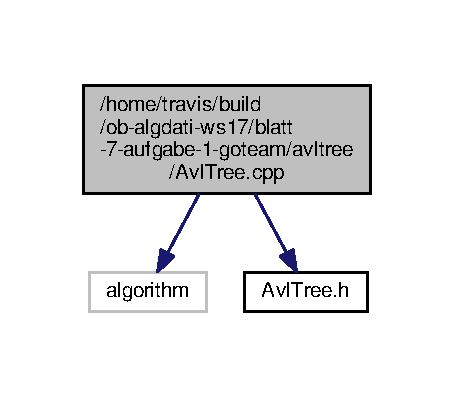
\includegraphics[width=218pt]{AvlTree_8cpp__incl}
\end{center}
\end{figure}
\subsection*{Functions}
\begin{DoxyCompactItemize}
\item 
Avl\-Tree\-::node $\ast$ \hyperlink{AvlTree_8cpp_ad7ffcf268628ee5a2dea0517021ca2ad}{find\-Sym\-Succ} (Avl\-Tree\-::node $\ast$node)
\end{DoxyCompactItemize}


\subsection{Function Documentation}
\hypertarget{AvlTree_8cpp_ad7ffcf268628ee5a2dea0517021ca2ad}{\index{Avl\-Tree.\-cpp@{Avl\-Tree.\-cpp}!find\-Sym\-Succ@{find\-Sym\-Succ}}
\index{find\-Sym\-Succ@{find\-Sym\-Succ}!AvlTree.cpp@{Avl\-Tree.\-cpp}}
\subsubsection[{find\-Sym\-Succ}]{\setlength{\rightskip}{0pt plus 5cm}Avl\-Tree\-::node$\ast$ find\-Sym\-Succ (
\begin{DoxyParamCaption}
\item[{Avl\-Tree\-::node $\ast$}]{node}
\end{DoxyParamCaption}
)}}\label{AvlTree_8cpp_ad7ffcf268628ee5a2dea0517021ca2ad}
Finding the symmetric successor.

This method finds the symmetric successor of the node given as a parameter.


\begin{DoxyParams}{Parameters}
{\em node} & the root of the tree \\
\hline
\end{DoxyParams}
\begin{DoxyReturn}{Returns}
the symmetric successor 
\end{DoxyReturn}

\hypertarget{AvlTree_8h}{\section{/home/travis/build/ob-\/algdati-\/ws17/blatt-\/7-\/aufgabe-\/1-\/goteam/avltree/\-Avl\-Tree.h File Reference}
\label{AvlTree_8h}\index{/home/travis/build/ob-\/algdati-\/ws17/blatt-\/7-\/aufgabe-\/1-\/goteam/avltree/\-Avl\-Tree.\-h@{/home/travis/build/ob-\/algdati-\/ws17/blatt-\/7-\/aufgabe-\/1-\/goteam/avltree/\-Avl\-Tree.\-h}}
}
This graph shows which files directly or indirectly include this file\-:
\nopagebreak
\begin{figure}[H]
\begin{center}
\leavevmode
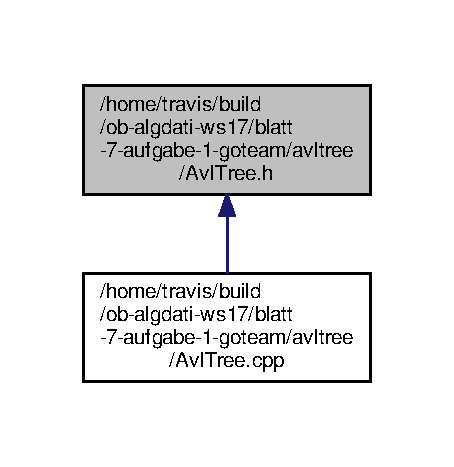
\includegraphics[width=218pt]{AvlTree_8h__dep__incl}
\end{center}
\end{figure}
\subsection*{Classes}
\begin{DoxyCompactItemize}
\item 
class \hyperlink{classAvlTree}{Avl\-Tree}
\begin{DoxyCompactList}\small\item\em The A\-V\-L Tree class. \end{DoxyCompactList}\end{DoxyCompactItemize}

%--- End generated contents ---

% Index
\newpage
\phantomsection
\addcontentsline{toc}{chapter}{Index}
\printindex

\end{document}
